\part{The language}\label{part:zilch}

\chapter{Introduction}\label{chap:zilch-introduction}

Low-level programming is programming with a few abstractions over the hardware.
For example, assembly languages mostly provide no or very little abstractions over CPU instructions (having one instruction set per target).
Functional programming is a kind of programming focused around functions and their composition.
However, because of this, many functional programming languages have a tendancy to be quite slow, at least compared to ``ordinary'' imperative programming languages.

\href{http://www.ats-lang.org/}{ATS} is one of those programming languages claiming to be both functional and quite low-level.
It compiles to C (therefore has a free FFI), has a complex dependent type system and many other things making it kind of great.
But ATS is hard to learn, because it has so much stuff\ldots

Yet Zilch is also a low-level functional programming language.
But the goal is to design a not-so-hard to learn programming language, while still having strong guarantees about the code written\footnote{When this was written, Zilch was far from production-ready, so most
of the guarantees have not yet been described here.}.
Prior knowledge about ML-style programming is still recommended before trying to tackle Zilch, but anybody without this kind of knowledge should also be able to learn Zilch fairly easily.

This part will try to describe and formalize (at least a bit, but some parts may be left informal) the Zilch programming language, going from the usual syntax onto the operational semantics.
Implementation details (such as error messages, program optimisations, \ldots) will not be covered by this document.

\section*{Some notes on the notation used}\label{sec:zilch-introduction-notation}

Zilch is really not a small programming language.
Because of that, sometimes we need some specific notation to described things like inference rules.

The mainly used notation is described here, but not necessarily everything will be described (sometimes, a little bit of common sense helps to understand).

\begin{itemize}
  \item Grammar
        \begin{figure}[H]
          \centering
          \scalebox{.5}{
            
\includegraphics{grammar-template-2}
          }
        \end{figure}
        \begin{itemize}
          \item Sharp rectangles describe that another rule is to be used there (the name of the rule is given in the rectangle);
          \item Rounded rectangles describe terminal tokens, i.e.\ pieces of string that must be litterally matched;
          \item The name of the grammar rule defined is given in the top-left corner of the diagram.
                A rule matches if and only if it is possible to go from the left to the right, only following the rails;
        \end{itemize}
\end{itemize}

\chapter{Grammar of Zilch programs}\label{chap:zilch-grammar}

A Zilch program is comprised of three different levels, each included in the next one:
\begin{itemize}
  \item The expression level, where an expression denotes a value which has a statically determined type;
  \item The declaration level, containing all function definitions, type definitions, type classes declarations, etc;
  \item The module level, where imports and module declarations live in;
\end{itemize}

\noindent Because it is not easy to materialize indentation properties in the grammar, it will instead be marked using the non-terminals\footnote{Those symbols are reserved and actually used as terminals, so we put them as non-terminals to remove any ambiguation.} \texttt{\{}, \texttt{\}} and \texttt{;}.
Note that these are not actually present in the source code, and are only a mean of hinting an indentation change.
\texttt{x \{ y; z \}} really means \texttt{x} followed by \texttt{y} which may be more indented or on the same line, and \texttt{z} which must be aligned with the beginning of \texttt{y}.
It therefore describes both layouts:

\noindent\begin{minted}{\zilchlexer}
  -- `y` on the same line as `x`:
  x y
    z
  -- or `y` on a new line:
  x
    y
    z
\end{minted}

\section{Lexicon}\label{sec:zilch-grammar-lexical}

This section describes the lexical structure of any Zilch program.
Note that the Unicode alternative syntax does not need to be supported, but makes the code look nicer.

\subsection{Identifiers, operators and reserved words}\label{subsec:zilch-grammar-lexical-identifiers}

Identifiers and operators are the same thing thanks to mixfix operators.
They are composed of only printable characters which are not considered special, and must not form keywords.

Mixfix operators also do not allow keywords as backbones (that is, \texttt{\_->\_} is not a valid mixfix operator because \texttt{->} is a keyword; however \texttt{\_->*\_} is valid because the backbone contains \texttt{->*}, not \texttt{->}).

\begin{figure}[H]
  \centering

  \scalebox{.5}{
    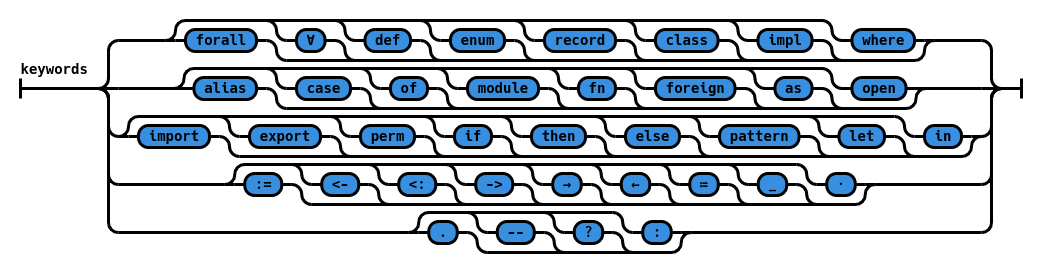
\includegraphics{zilch/lexicon/keywords}
  }
  \\
  \scalebox{.5}{
    
\includegraphics{zilch/lexicon/special}
  }
  \\
  \scalebox{.5}{
    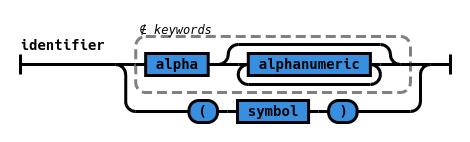
\includegraphics{zilch/lexicon/identifier}
  }

  \caption{Lexical units for identifiers.}
  \label{fig:zilch-grammar-lexical-identifiers-grammar}
\end{figure}

\subsection{Whitespaces}\label{subsec:zilch-grammar-lexical-whitespaces}

Whitespace tokens are basically word separators.
Because of that, comments are also counted as whitespaces, despite not really being an invisible sequence.
However, because of how mixfix operators are parsed, the sequence \verb|_--_...| corresponds to the two tokens \verb|<underscore>| and \verb|<comment _...>|, not \verb|<identifier _--_...>| (same goes for any mixfix operator that has \verb|--| as a backbone; but again, \verb|_--*_| \textit{is a valid operator}).

\begin{figure}[H]
  \centering

  \scalebox{.5}{
    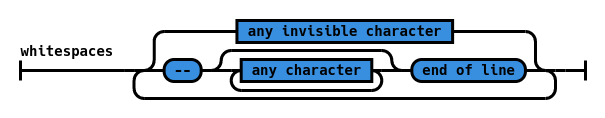
\includegraphics{zilch/lexicon/whitespaces}
  }

  \caption{Whitespace lexical units.}
  \label{fig:zilh-grammar-lexical-whitespaces-grammar}
\end{figure}

